\documentclass[11pt,t]{beamer}
\usepackage[utf8]{inputenc}
\usepackage[T1]{fontenc}
\usepackage{lmodern}
\usepackage{graphicx}
\usepackage{pgfplots}
\usepackage[french]{babel}
\usepackage{listings}
\usepackage{listingsutf8}
\usetheme{Madrid}

\begin{document}
	\author[J.Delaeter C.Ghyselinck]{Joseph \bsc{Delaeter} et Corentin \bsc{Ghyselinck}}
	\title{Projet Openxum}
	\subtitle{Presentation orale 1}
	\logo{
\includegraphics[width=45pt]{images/logoulco.pdf}}
	%\institute{}
	%\date{}
	%\subject{}
	%\setbeamercovered{transparent}
	%\setbeamertemplate{footline}[frame number]
	\setbeamertemplate{navigation symbols}{}
	
	\subject{java}
	\keywords{java, programmation, orientée, objet}
	
	\AtBeginSection{
		\begin{frame}
			\frametitle{Plan du cours}
			\tableofcontents[currentsection, hideothersubsections]
		\end{frame}
	}

	\AtBeginSubsection{
		\begin{frame}
			\frametitle{Plan du cours}
			\tableofcontents[currentsubsection]
		\end{frame}
	}

	\lstset{aboveskip=1ex, language=Java, basicstyle=\ttfamily, breaklines, keywordstyle=\color{blue}, commentstyle=\color{gray}\itshape, stringstyle=\color{orange}}
	
	\newenvironment<>{remarque}{
		\setbeamercolor{block title}{bg=orange}
		\begin{block}{Remarque}
			
	}
	{
		\end{block}
	}

	\newenvironment<>{syntaxe}{
		\setbeamercolor{block title}{bg=cyan}
		\begin{block}{Syntaxe}
			
		}
		{
		\end{block}
	}
	
	\begin{frame}[plain]
		\maketitle
		\begin{abstract}
			Document réalisé à partir du cours de M\up{r} Grégory \bsc{Bourgin}: bourguin@lisic.univ-littoral.fr
		\end{abstract}
	\end{frame}

	\begin{frame}
		\frametitle{Plan du cours}
		\tableofcontents
	\end{frame}

	\chapter{Présentation du langage}
		\section{Qu'est-ce que le \lang{} ?}
			
				Simula 67 a été conçu par une équipe scandinave et a été
				publié en 1967.
				
				Au début des années 70, Alan Kay conçoit au PARC (Rank
				Xerox) le langage SmallTalk, qui est encore aujourd'hui \emph{la} référence dans les langages orientés objet.
				
				A la fin des années 70 et au début des années 80, on assiste à la naissance de nombreuses extensions objet d'anciens langages : Object Pascal, Objective C, C++, CLOS, ADA...
				
				Au milieu des années 90, Sun publie Java. Ses qualités
				intrinsèques et le fait qu'il soit particulièrement adapté à
				Internet en font immédiatement un standard.
				
				Une énorme masse de documentation peut être trouvée sur
				Internet.		
				
				Le \lang{} est:
				\begin{itemize}
					\item Un langage orienté objet (\emph{POO}\footnote{Programmation Orientée Objet})
					\item Une architecture \emph{Virtual Machine}
					\item Un ensemble d'API variées
					\item Un ensemble d'outils: le \emph{JDK\footnote{Java Development Kit}}
					\item Portable:
						\begin{itemize}
							\item La compilateur \lang{} génère du langage \emph{byte code}
							\item La \emph{JVM}\footnote{Java Virtual Machine} est présente sur la majeure partie des systèmes d'exploitation Windows, Mac, Unix...
							\item Il dispose d'une sémantique très précise
							\item Il supporte un code écrit en \emph{Unicode}
							\item Il est accompagné d'une librairie standard
						\end{itemize}	
					\item Robuste:
						\begin{itemize}
							\item Orienté à l'origine pour des applications embarquées
							\item Gère la mémoire par \emph{garbage collector}
							\item Dispose d'un mécanisme d'\emph{exceptions}
							\item Convertissions sûres automatiques uniquement
							\item Contrôle des \emph{cast} à l'exécution
						\end{itemize}
				\end{itemize}
				
				\attention{
					\begin{itemize}
						\item Le \lang{} n'est pas du JavaScript, car le \lang{} est un langage généraliste, contrairement au JavaScript qui est un langage orienté sur la programmation Web !
						\item Le \lang{} n'est pas du C++ ! \lang{} est un langage objet purement objet, et de plus haut niveau.
					\end{itemize}	
				}	
		
		\section{Les outils}
		
			Pour programmer en \lang{} sur ordinateur, nous utiliserons l'un des environnements de développement (\emph{IDE}) suivant:
				\begin{itemize}
					\item SunJDK (compilateur, interpréteur...)
					\item Eclipse (gratuit)
					\item IntelliJ (version \og community\fg{} gratuite, mais version commerciale payante)
					\item NetBeans
				\end{itemize}
			Liste des outils utilisés dans la programmation \lang{}:
				\begin{description}
					\item[javac:] compilateur de sources Java
					\item[java:] interpréteur de byte code
					\item[appletviewer:] interpréteur d'applet
					\item[javadoc:] générateur de documentation (HTML, MIF)
					\item[javah:] générateur de header pour l'appel de méthodes natives
					\item[javap:] désassembleur de byte code
					\item[jdb:] debugger
					\item[javakey:] générateur de clés pour la signature de code
				\end{description}
			Liste des \emph{API} standards:
				\begin{description}
					\item[java.lang:] types de bases, etc.
					\item[java.util:] HashTable, Vector, Stack, Date...
					\item[java.io:] accès aux entrées/sorties par flux
					\item[java.net:] socket, URL...
					\item[java.sql:] accès homogène aux bases de données
					\item[java.security:] signatures, cryptographie, authentification...
				\end{description}
		
		\section{Références}
		
			\lang{} dispose d'un grand nombre de ressources sur internet. A l'heure actuelle, nous sommes à la 8\ieme{} version de \lang{}: \url{https://docs.oracle.com/javase/8/}
	
%	\section{Les éléments du langage}

	\subsection{Types primitifs}
	
		\begin{frame}
			\frametitle{Les éléments du langage}
			\framesubtitle{Types primitifs}
			Tableau des types primitifs:
			\begin{center}
				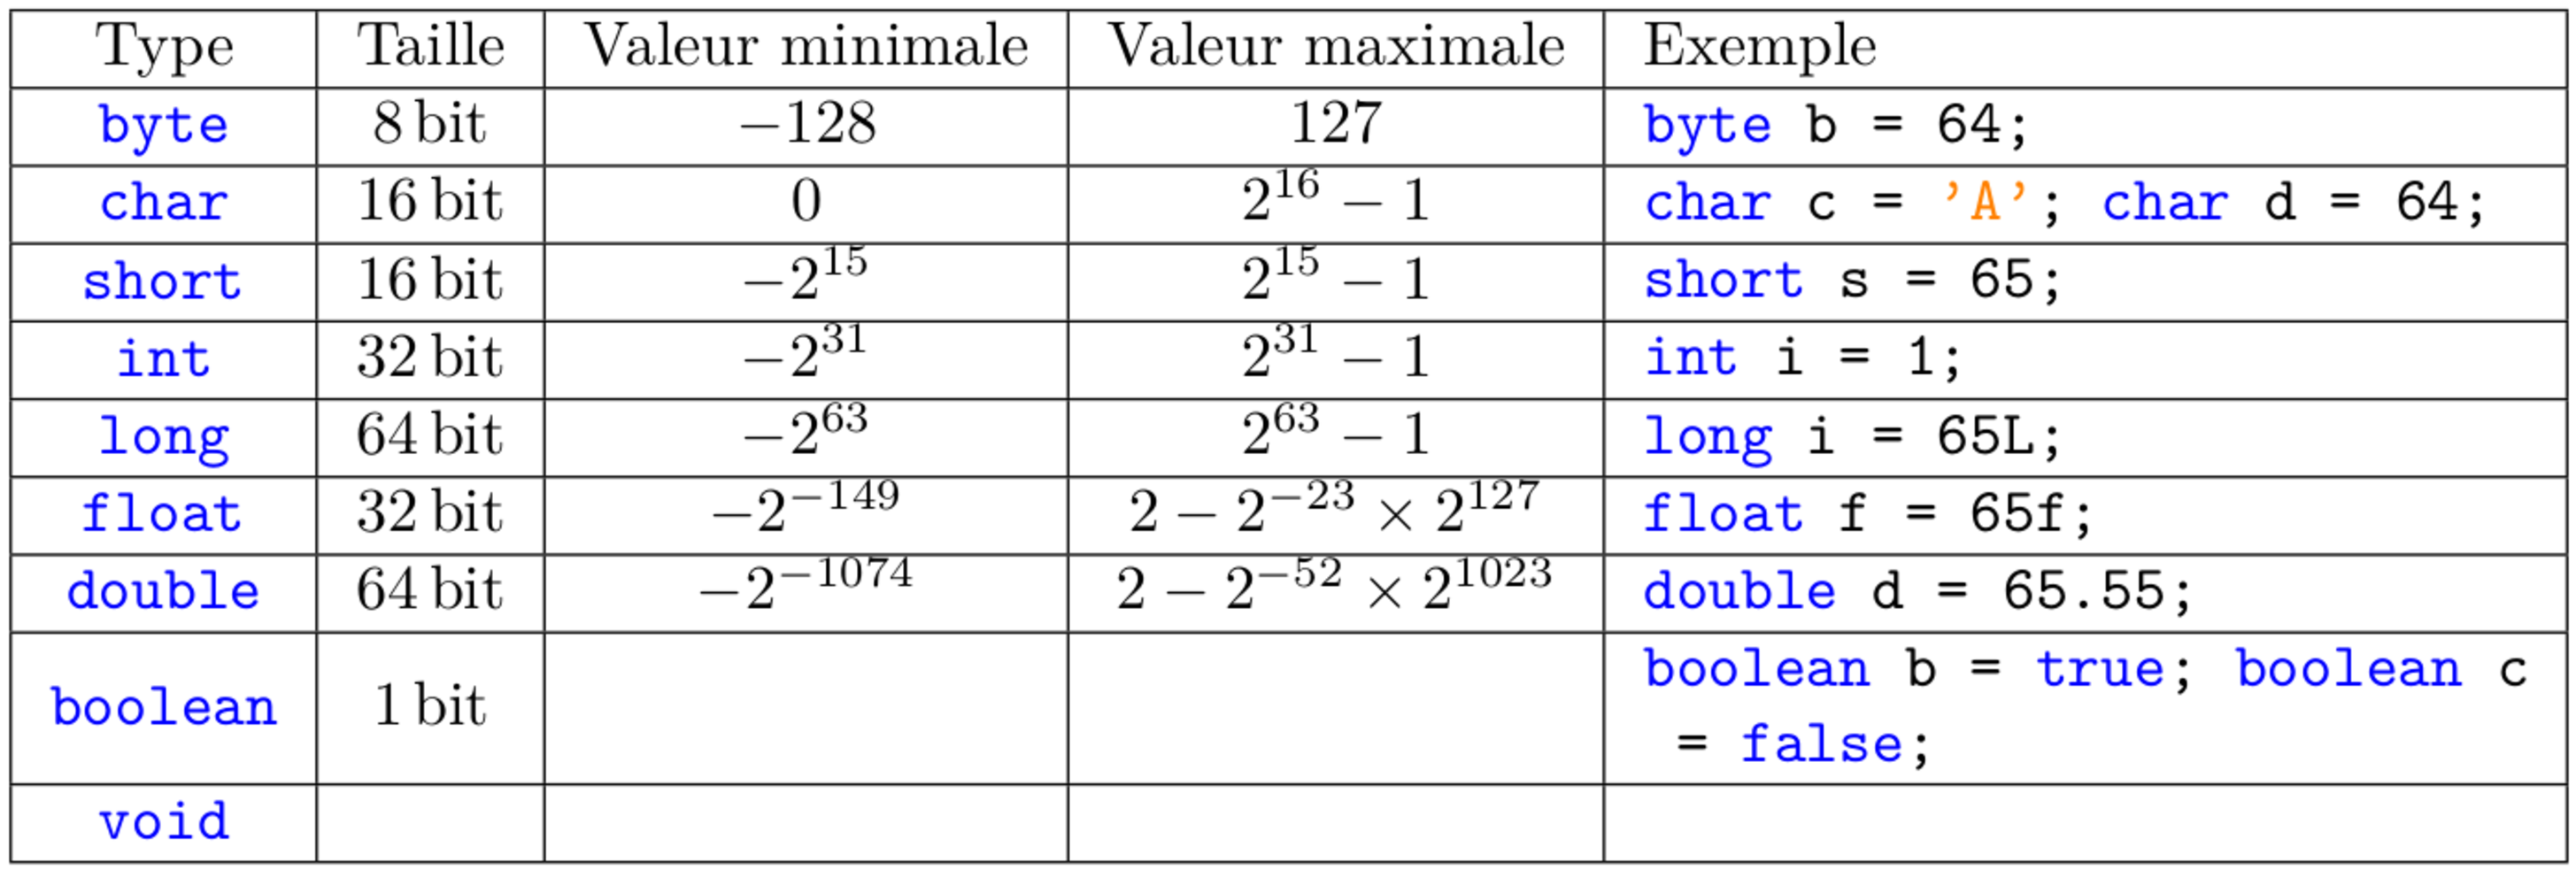
\includegraphics[width=1.0\linewidth]{images/typesprimitifs}
			\end{center}
		\end{frame}
			
	
	\subsection{Variables}
	
		\begin{frame}[fragile]
			\frametitle{Les éléments du langage}
			\framesubtitle{Variables}
			\begin{fact}
				En Java, les variables sont typées, et peuvent être déclarées dans n'importe quel bloc du code.
			\end{fact}
			\pause{}
			\begin{columns}
				\begin{column}{0.45\textwidth}
					\begin{example}
						\lstinputlisting{code/porteevariables.java}
					\end{example}
				\end{column}
				\begin{column}{0.45\textwidth}
					\pause{}
					\begin{block}{Résultat}
						La variable \lstinline|x| sera utilisable dans \visible<4->{\textcolor{purple}{les blocs 1 et 2}.}
						
						La variable \lstinline|y| sera utilisable \visible<5->{\textcolor{purple}{uniquement dans le bloc 2}.}
					\end{block}
				\end{column}
			\end{columns}
		\end{frame}
	
		\begin{frame}[fragile]
			\frametitle{Les éléments du langage}
			\framesubtitle{Variables}
			
			\begin{block}{Opérateurs d'affectation}
				\begin{itemize}
					\item \lstinline|=|
					\item \lstinline|+=|
					\item \lstinline|-=|
					\item \lstinline|*=|
					\item \lstinline|/=|
					\item \lstinline|%=|
				\end{itemize}
			\end{block}		
		\end{frame}
	
	\subsection{Expressions}
	
		\begin{frame}[fragile]
			\frametitle{Les éléments du langage}
			\framesubtitle{Expressions}
			\begin{definition}
				Une \emph{expression ternaire} est une notation \og simplifiée\fg{} d'un \emph{test logique}.
			\end{definition}
			\begin{columns}
				\begin{column}{0.45\textwidth}
					\pause{}
					\begin{example}[Test classique]
						\lstinputlisting{code/testClassique.java}
					\end{example}
				\end{column}
				\begin{column}{0.45\textwidth}
					\pause{}
					\begin{example}[Test ternaire]
						\lstinputlisting{code/operateurTernaire.java}
					\end{example}
				\end{column}
			\end{columns}	
		\end{frame}
	
		\begin{frame}[fragile]
			\frametitle{Les éléments du langage}
			\framesubtitle{Expressions}
			\begin{alertblock}{Attention !}
				Il est nécessaire de \emph{caster} des affectations lorsque celles-ci ne sont pas implicites, sinon des erreurs de compilation sont détectées.
			\end{alertblock}
			\pause{}
			\begin{example}
				\lstinputlisting{code/cast.java}
			\end{example}
			
		\end{frame}
	
		\begin{frame}[fragile]
			\frametitle{Les éléments du langage}
			\framesubtitle{Expressions}

			\begin{remarque}
				Levé d'ambiguité entre \lstinline|float| et \lstinline|double|:
				\lstinputlisting{code/floatdouble.java}
			\end{remarque}
		\end{frame}
	
	\subsection{Méthodes}
	
		\begin{frame}[fragile]
			\frametitle{Les éléments du langage}
			\framesubtitle{Méthodes}
			
			\begin{definition}
				Une \emph{méthode} est une fonction appartenant à une classe.
			\end{definition}
			\pause{}
			\begin{syntaxe}
				\lstinputlisting{code/basemethode.java}
			\end{syntaxe}
		\end{frame}
	
		\begin{frame}[fragile]
			\frametitle{Les éléments du langage}
			\framesubtitle{Méthodes}
			
			\begin{remarque}
				\begin{enumerate}
					\item \uncover<2,5->{Le type de retour est un type primitif, une classe ou \lstinline|void|.}
					\item \uncover<3,5->{La liste des paramètres peut être vide.}
					\item \uncover<4,5->{Si le type de retour n'est pas un \lstinline|void|, la fonction doit se terminer par un \lstinline|return|.}
				\end{enumerate}
			\end{remarque}
			\uncover<5->{
				Passage de paramètres:
				\begin{description}
					\item[Type simple:] passés \emph{par valeur} \alert{uniquement}
					\item[Type objet ou tableaux:] passés \emph{par référence}
				\end{description}
			}
		\end{frame}
	
	\subsection{Structures de contrôle}
	
		\begin{frame}[fragile]
			\frametitle{Les éléments du langage}
			\framesubtitle{Structures de contrôle (IF)}
			\begin{fact}
				Le code à l'intérieur d'un \lstinline|if| s'exécute uniquement si la condition est vraie.
			\end{fact}
			\pause{}
			\begin{alertblock}{Attention !}
				Plusieurs notations sont possibles ! Soyez vigilants au nombre de lignes de code dans votre bloc d'instructions (si votre condition est vraie) pour bien choisir la notation.
			\end{alertblock}
			\pause{}
			\begin{syntaxe}
				\begin{itemize}[<+->]
					\item \lstinline|if(condition) {...} else {...}|
					\item \lstinline|if(condition) instruction;|
					\item \lstinline|if(condition) instruction; else instruction;|
					\item \lstinline|if(condition) instruction; else {...}|
					\item \lstinline|if(condition) {...} else instruction;|
				\end{itemize}
			\end{syntaxe}
		\end{frame}
	
		\begin{frame}[fragile]
			\frametitle{Les éléments du langage}
			\framesubtitle{Structures de contrôle (IF)}
			\begin{example}
				\lstinputlisting{code/exempleIF.java}
			\end{example}
		\end{frame}
	
		\begin{frame}[fragile]
			\frametitle{Les éléments du langage}
			\framesubtitle{Structures de contrôle (WHILE)}
			\begin{fact}
				Le code à l'intérieur d'un \lstinline|while| s'exécute tant que la condition est vraie.
			\end{fact}
			\pause{}
			\begin{syntaxe}
				\begin{itemize}
					\item \lstinline|while(condition) {...}|
					\item \lstinline|while(condition) instruction;|
				\end{itemize}
			\end{syntaxe}
			\pause{}
			\begin{example}
				\lstinputlisting{code/exempleWHILEsansDO.java}
			\end{example}
		\end{frame}
	
		\begin{frame}[fragile]
			\frametitle{Les éléments du langage}
			\framesubtitle{Structures de contrôle (WHILE)}
			\begin{remarque}
				Le \lstinline|while|, tel que définit jusqu'à présent, vérifie la condition avant d'exécuter (au moins une fois) les instructions. 
				
				Dans certains cas, il peut être utilise d'exécuter les instructions au moins une fois, avant de vérifier si il faut les répéter.
			\end{remarque}
			\pause{}
			On utilisera l'instruction: \lstinline|do|.
			\pause{}
			\begin{syntaxe}
				\lstinline|do{ ... } while(condition)|
			\end{syntaxe}
			
		\end{frame}
	
		\begin{frame}[fragile]
			\frametitle{Les éléments du langage}
			\framesubtitle{Structures de contrôle (DO ... WHILE)}
			\begin{example}
				\lstinputlisting{code/exempleWHILEavecDO.java}
			\end{example}
			\pause{}
			\begin{remarque}
				Sans l'instruction \lstinline|do|, aucune instruction ne se serait exécutée.
			\end{remarque}
			
		\end{frame}
	
		\begin{frame}[fragile]
			\frametitle{Les éléments du langage}
			\framesubtitle{Structures de contrôle (FOR)}
			\begin{fact}
				Le code à l'intérieur d'une boucle \lstinline|for| s'exécute un nombre défini de fois.
			\end{fact}
			\pause{}
			\begin{syntaxe}
				\begin{itemize}
					\item \lstinline|for(initialisation, condition, incrementation) { ... }|
					\item \lstinline|for(initialisation, condition, incrementation) instruction;|
				\end{itemize}
			\end{syntaxe}
			Avec:
			\pause{}
			\begin{description}[<+->]
				\item[initialisation:] initialisation de la / les variable(s) de boucle
				\item[condition:] la boucle sera répétée tant que la condition sera vraie
				\item[incrementation:] incrémente la variable de boucle
			\end{description}
			
		\end{frame}
	
		\begin{frame}[fragile]
			\frametitle{Les éléments du langage}
			\framesubtitle{Structures de contrôle (FOR)}
			\begin{example}
				\lstinputlisting{code/exempleFOR.java}
			\end{example}
			\pause{}
			\begin{alertblock}{Attention !}
				Ce programme affiche les nombres de 0 à 9, et non jusqu'à 10 !
			\end{alertblock}
		\end{frame}
	
		\begin{frame}[fragile]
			\frametitle{Les éléments du langage}
			\framesubtitle{Structures de contrôle (SWITCH)}
			\begin{definition}
				Un \lstinline|switch| est un bloc contenant une succession de tests. On peut le comparer à une succession de \lstinline|if|.
			\end{definition}
			\pause{}
			\begin{itemize}
				\item Structure très utile pour effectuer beaucoup de tests avec la même variable.
				\item Elle évite d'écrire un programme avec une succession de tests en \lstinline|if| qui utilisent \alert{la même} variable d'entrée. 
			\end{itemize}
			
		\end{frame}
	
		\begin{frame}[fragile]
			\frametitle{Les éléments du langage}
			\framesubtitle{Structures de contrôle (SWITCH)}
			\begin{syntaxe}
				\lstinputlisting{code/syntaxeSwitch.java}
			\end{syntaxe}
			
		\end{frame}
	
		\begin{frame}[fragile]
			\frametitle{Les éléments du langage}
			\framesubtitle{Structures de contrôle (BREAK et CONTINUE)}
			\begin{remarque}
				Il peut être utile:
				\begin{enumerate}
					\item <2-> d'arrêter une boucle avant sa fin
					\item <3-> de passer automatiquement à l'itération suivante sans exécuter les instructions qui suivent dans le bloc
				\end{enumerate}
			\end{remarque}
			\visible<4->{
				Pour cela, on utilisera respectivement les instructions suivantes:
				\begin{enumerate}
					\item <5->\lstinline|break;|
					\item <6->\lstinline|continue;|
				\end{enumerate}
			}
			
		\end{frame}
	
	\section{Suppléments \LaTeX}

	\begin{frame}
		\frametitle{Suppléments \LaTeX}
		\framesubtitle{Graphique}
		\begin{tikzpicture}
			\begin{axis}[domain=0:360, no markers, xlabel=$x$, ylabel=$f(x)$]
			\addplot {cos(x)};
			\addplot {sin(x)};
			\addplot {tan(x)};
			\legend{$cos(x)$, $sin(x)$,$tan(x)$}
			\end{axis}
		\end{tikzpicture}
		
	\end{frame}


\end{document}